\documentclass[10pt,twocolumn]{article}
\usepackage{times}
\usepackage{url}

% do not change these values
\baselineskip 12pt
\textheight 9in
\textwidth 6.5in
\oddsidemargin 0in
\topmargin 0in
\headheight 0in
\headsep 0in

\usepackage{graphicx}
\usepackage{subcaption}

\begin{document}

\title{Title}
\author{Zhouwang Fu$^1$ and Zhengwei Qi$^1$ \\
% \small {\em  $^1$Shanghai Jiao Tong University \quad
%           $^2$Cloud National Labs} \\ [2mm]
\small {\em  $^1$Shanghai Jiao Tong University} \\ [2mm]
% \small Submission Type: Research
}
\date{}
\maketitle

\begin{abstract}
Shuffle is the term used to descirbe the cross-network read and aggregation
of partitioned ancestor data before invoking reduce operation.
As DAG computing framworks keep evolving, calculation and scheduling of each task are well optimized. 
However shuffle cuts off the data processing pipeline, introduce significant latency to successors.
To remove shuffle overhead, we present XXX, a plugin system to decouple shuffle from DAG computing 
framework. XXX captures shuffle data in the memory and uses heuristic-FIFO scheduling to balance data
blocks to elimite the explict barrier. We implement XXX and change Spark to use XXX as external shuffle 
 service and scheduler. We evaluate XXX performance both on simulation and 50-machine Amazon EC2 cluster.
 Results show that, by incorporating XXX in Spark, the shuffle overhead can be reduce XXX.

\end{abstract}

\section{Introduction}

\section{Motivation}
In this section, we first study the shuffle pattern (\ref{shuffle pattern}) . 
Then we show the observations of the opportunities to optimize shuffle in \ref{observation}
\subsection{Characteristic of Shuffle} \label{shuffle pattern}

In large scale data parallel computing, enormous datasets are partitioned into pieces to fit the memory of each node since the very beginnig of MapReduce\cite{mapreduce}.
Meanwhile, complicated application procedures are divided into steps. The successor steps take the output of ancestors as input to do the computation. Shuffle occurs when each successor needs 
part of data from all ancestors' output. In order to provide a clear illustration, we define those computing each partition of data in one step as task. For tasks that generates shuffle output, we call
them map task. For tasks that consume shuffle output, we call them reudce tasks. Note that one task may have both shuffle data generation and consumption, we call it intermediate task.

Shuffle is designed to achieve an all-to-all data blocks transfer among nodes in cluster. It exists in both MapReduce models and DAG computation models.

Shuffle mainly contains two phases itself: \textbf{Data Partition} and \textbf{Data Transfer}. For \textbf{Data Partition}, each map task and intermediate task will partition the result data (key, value pair) into several buckets according to the partition function.
The buckets number equals to the number of tasks in the next step. When the map tasks and intermediate tasks finish, all the shuffle output data will be written into local persistent storage for fault tolerance \cite{mapreduce, spark}.
\textbf{Data Transfer} starts at the begnning of reduce tasks and intermediate tasks. These tasks will fetch the data that belongs to their corresponding partitions from both remote nodes and local storage.

In short, shuffle is loosely coupled with application context and it's I/O intensive.

Since intensive I/O operation will be triggered during a shuffle, this can introduce a significant lantency to the application. Reports show that, 60\% of MapReduce jobs at Yahoo
and 20\% at Facebook are shuffle intensive workloads\cite{shufflewatcher}. For those shuffle intensive jobs, the shuffle lantency may even dominate Job Completion Time. 
For instance, a MapReduce trace analysis from Facebook shows that shuffle accounts for 33\% JCT on average, up to 70\% in shuffle intensive jobs\cite{managing}.
Meanwhile, the completion time of shuffle correlates with the performance of storage devices, network and even applications. 
This variation may bring a huge challenge for operators to find the correct configuration of the DAG framework.

\subsection{Observation} \label{observation}
Of course, shuffle is unavoidable in a DAG computing process. But \textit{can we mitigate or even remove the overhead of shuffle?} To find the answers, we run some representative applications on a Spark in a 5 m4.xlarge Aamzon EC2 cluster. We than capture and plot the CPU utilization, I/O throughput and tasks execution information on each node. Take the trace in Figure \ref{fig:util} as an example, which is caputured during one Spark GroupByTest job. This job has 2 rounds of tasks for each node. We mark the 'Execution' phase in the figure from the launch time of the first task on this node to the execution finish timestamp of the last one. The 'Shuffle Write' phase is marked from the timestamp of the begining of the first partitioned data write. The 'Shuffle Read and Execution' phase is mark from the start of the first reduce launch timestamp.
Figure \ref{fig:util} contains data including two stages connected by one shuffle. By analyzing the trace combing with Spark, we propose following observations.
\begin{figure*}
	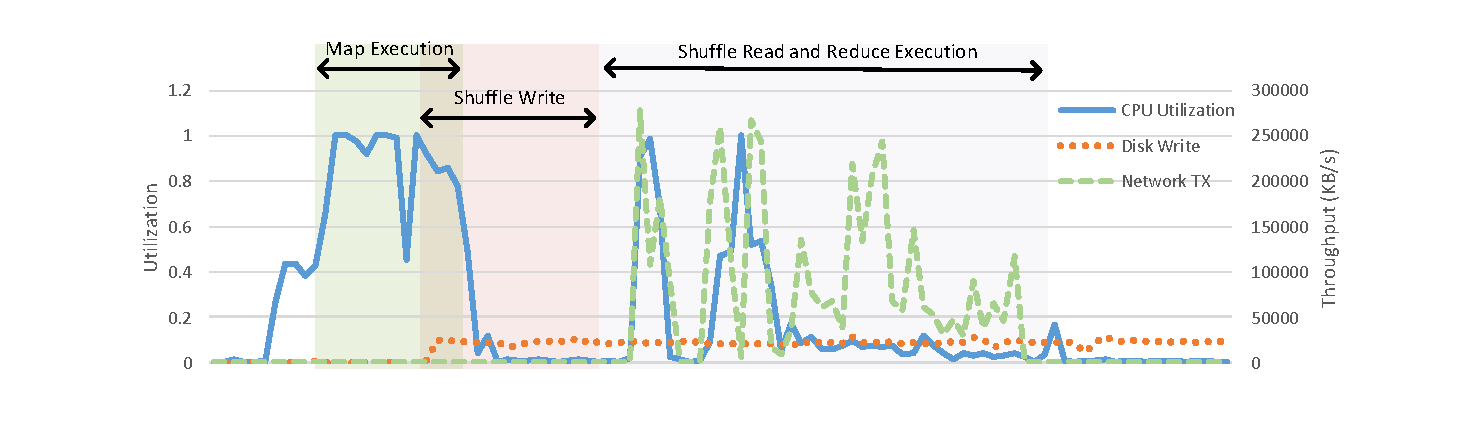
\includegraphics[width=\textwidth]{fig/util}
	\caption{CPU utiliazation and I/O throughput of a node during a Spark single shuffle application}
	\label{fig:util}
\end{figure*}

\subsubsection{Multi-rounds tasks in each stages}
Both experiece and DAG framework manuals recommand that multi-rounds execution of each stage will benifit the performance of whole application.
For example, Hadoop MapReduce Tutorial \cite{hadooptutorial} suggests that \textit{10-100 maps per-node} and \textit{0.95 or 1.75 $\times$ no. of nodes $\times$ no. of maximum container per node} seem to be the right level of parallelism. 
In Spark, the memory available to each task(partition) roughly equals to \textit{spark.executor.memroy $\times$ spark.memory.fraction}\cite{sparkconf}. 
We have two rounds of tasks in job of Figure \ref{fig:util} to process about 70GB data. Figure \ref{fig:util} shows that the second phase of shuffle -- \textbf{Data Transfer} will start until the reduce stage starts.
But the shuffle data will become available as soon as the execution of one task is finished. Though in the context of Spark, the reduce task can do compuation while fetchin data, the uncontrolled network congestion may still hurt the performance. However, if the destination of the shuffle output of each task is aware, the property of mutil-round can be leveraged to do \textbf{Data Transfer} ahead of reduce stage.

\subsubsection{Tight copule between shuffle and computation}
Another information we get from the trace is that shffle should be decoupled from task which is a execution unit in both Spark and Hadoop MapReduce. In general, CPU and memory are binded as a schedule slot in DAG resource scheduler. When a task is scheduled to a slot, it won't release until it reaches the end of task. In Figure \ref{fig:util}, the resource of Spark executor will be realsed at the ending of 'Shffle Write'.
But CPU becomes idle almost as soon as the 'Exectuion' is finished. On the other hand, shuffle is I/O intensive job. It doesn't involved CPU and application context. If the shffle can be decopled from task, the slot can be relased after 'Execution' phase. The early release can benifit other tasks to achieve better overall performance of the DAG framework.

\subsubsection{I/O performance varys}
When we look into the performance of disk and network in our test case, there is huge variance. Since we use the standard EBS as our backend storage for the EC2 instances, the I/O performance of disk is poor. 
At the same time, the exclusive bandwidth of each instance is 750 Mbps\cite{aws}. In this case, the bottleneck of shuffle is disk, which introduces a significant latency for the application. Vice versa, in some cases, the congestion of network may also become the bolltle of shuffle\cite{varys}. The uncertainty of the I/O performance cause a huge challenge for optmizing the DAG computing in the cluster. For network latency, the most we can do is to mitigate the transfer delay. As for disk write, we believe it's not necessary for today's cluster. Recall that the persistence of shuffle data is used only for reduce fault tolerence, but mean time to failure(MTTF) for a server is counted in the scale of year\cite{tachyon}. In addition, we believe combing the high speed of network and memory is a better choice for fault tolerence. We will present more details in Section \ref{design}.

\subsubsection{Shuffle size is small}
	\begin{figure}
	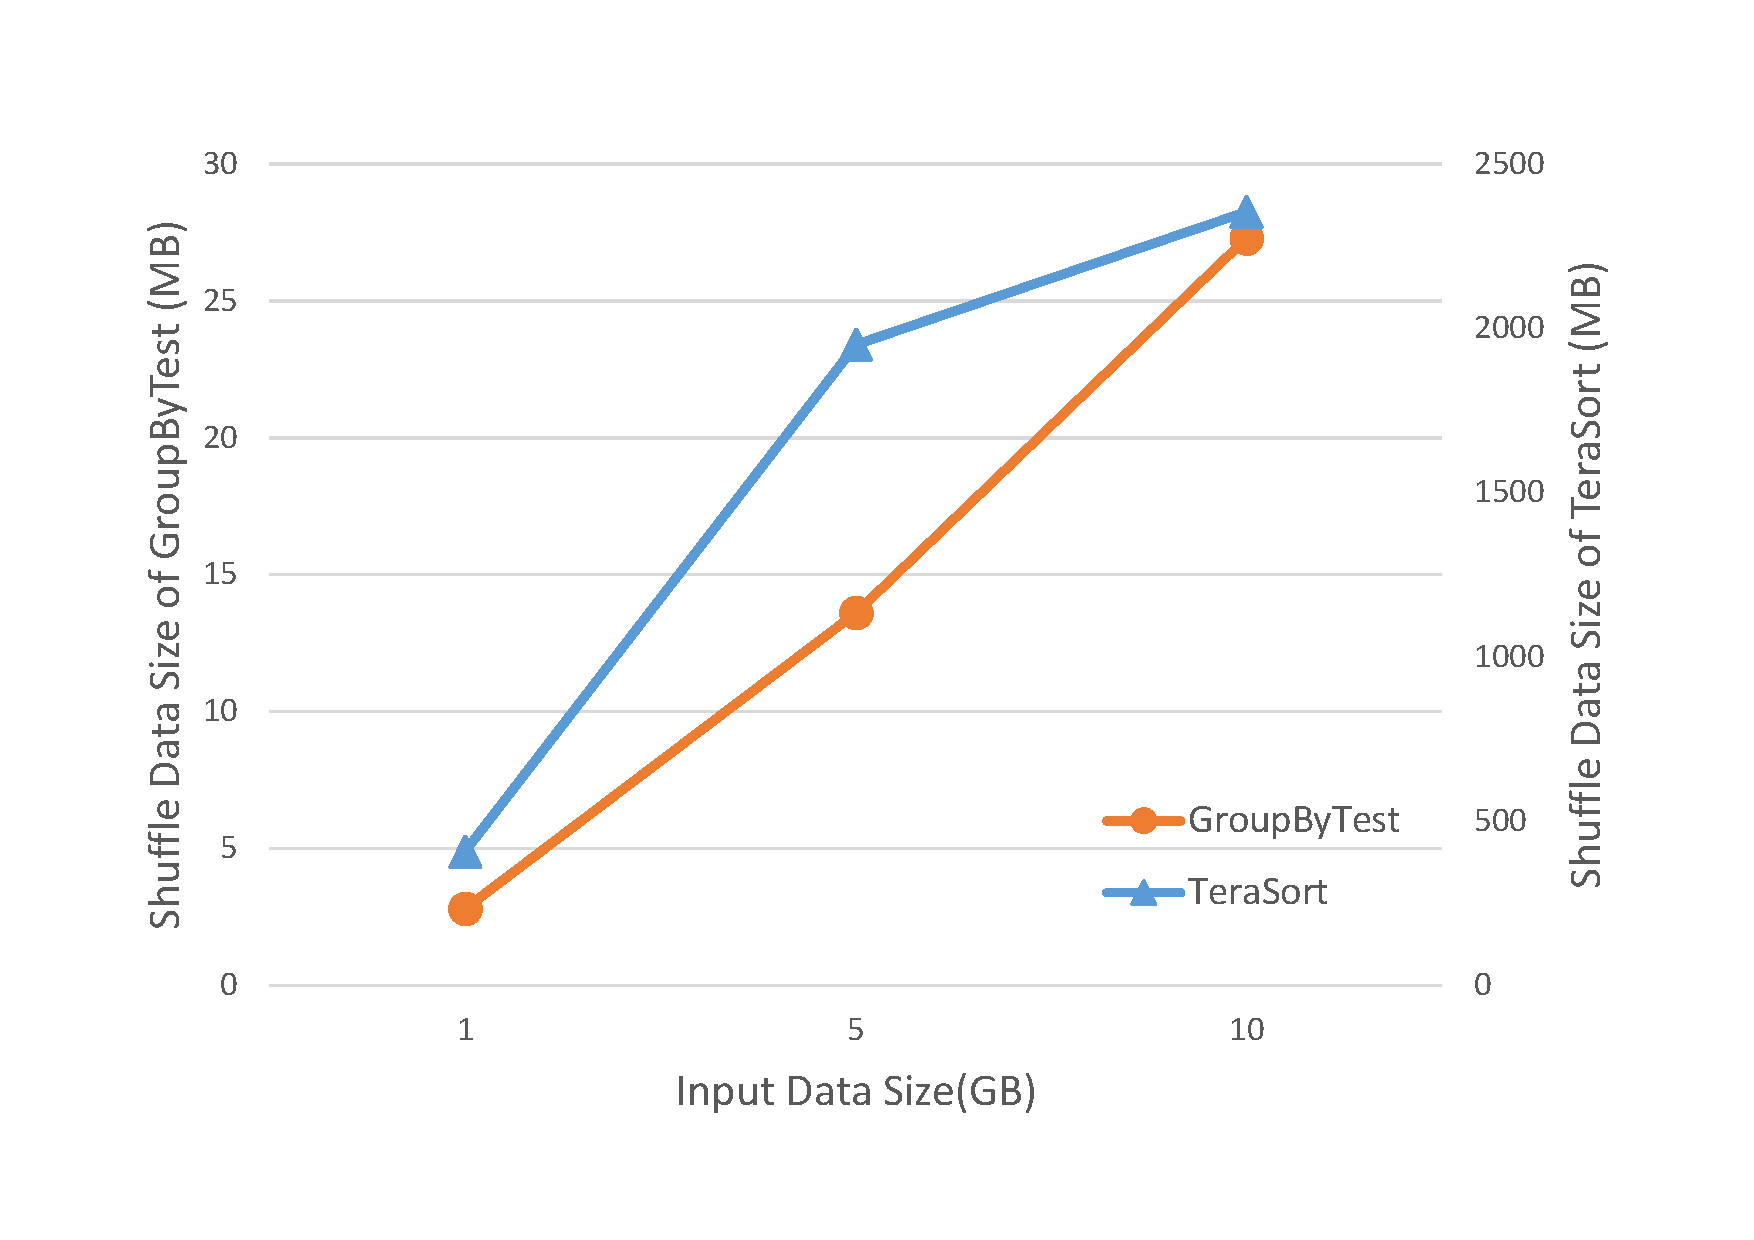
\includegraphics[width=\linewidth]{fig/shuffle_size}
	\caption{Shuffle Size Comparing with Input Size}
	\label{fig:shuffle_size}
\end{figure}
In order to accelearte computation, Spark will put all the input data set for a task into memroy. Comparing to the input dataset, size of shuffle data is relatively small. We persent to typical application on Spark to show the releationship between shuffle data comparing with the inpu dataset in Figure \ref{fig:shuffle_size}. Although TeraSort\cite{terasort} is known as a shuffle intensive job, in a 10GB input TeraSort, the shuffle size is less than 3GB. When it's mapped to a 5 nodes cluster, it only taks about 500MB memory (~25\% of input size for each node) to cache the shuffle data in memory. This is another reason that disk should not be involved in the whole shuffle procedure.


Based on these observations, it's straightforward to come up with a optimization to use memory to store the shuffle data and overlap the I/O operations of shuffle
by leveraging multi-rounds property of DAG computing. In order to achieve this optimization, we have to decouple shuffle from task and 
perform pre-fetch as soon as each output of map task and intermediate task is available. But is this feasible? We try to answer this question
in the following sections.

\section{Achieve Shuffle Optimization}
In this section, we try to achieve shuffle optimization by applying
\begin{itemize}
	\item Decouple shuffle from task
	\item Pre-fetch shuffle to reduce node
\end{itemize}
on the DAG computing framwork.
We choose Spark as the representative of DAG computing framwork to implement our optimization.
\subsection{Decouple shuffle from task}
On the map task side of shuffle, it's used to partition the output of map task according to the pre-defined partitioner. More specifically, shuffle takes a set of key-value pairs as input. And than it calculates the partitioner number of a key-value pait by applying pre-defined the partition function to the key. At last it put the key-value pair into the coressponding parition. The output at last is a set of blocks. Each of them contains the key-value pairs for one partition. For those application context unrelated blocks, they can be easily hijacked in the memory of Spark executor and moved out of JVM space via memory mapping. Meanwhile, we have to prevent the memory spill during the shuffle partition procedure, so that the shuffle data can never touch the disk. The default shuffle spill threshold in Spark is 5GB\cite{sparksource}, which is big enough in most scenarios according to Figure \ref{fig:shuffle_size}.
\begin{figure*}
	\centering
	\begin{subfigure}[b]{0.32\linewidth}
		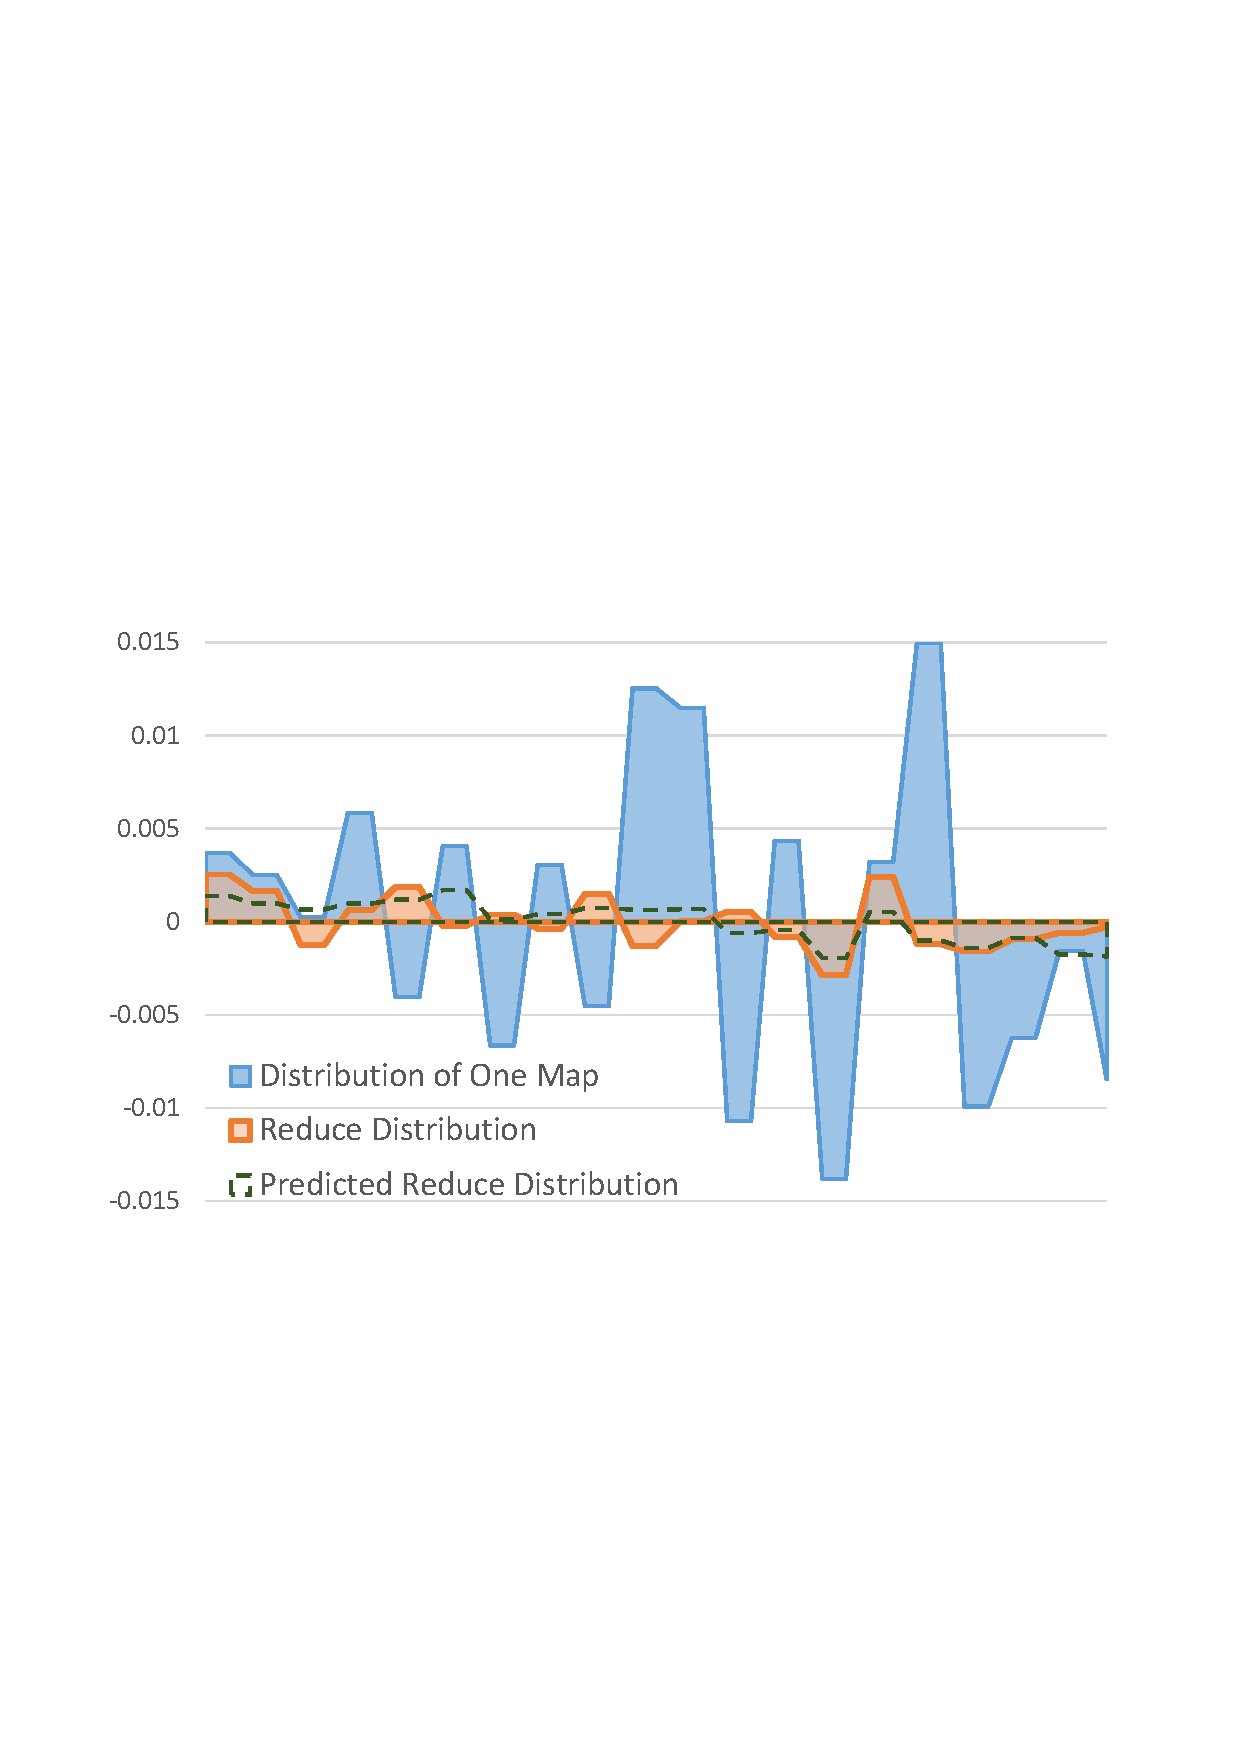
\includegraphics[width=\linewidth]{fig/hash_pre}
		\caption{Reduce Distribution of Hash Parition in Random Dataset}
		\label{fig:hash_pre}
	\end{subfigure}
	\begin{subfigure}[b]{0.32\linewidth}
		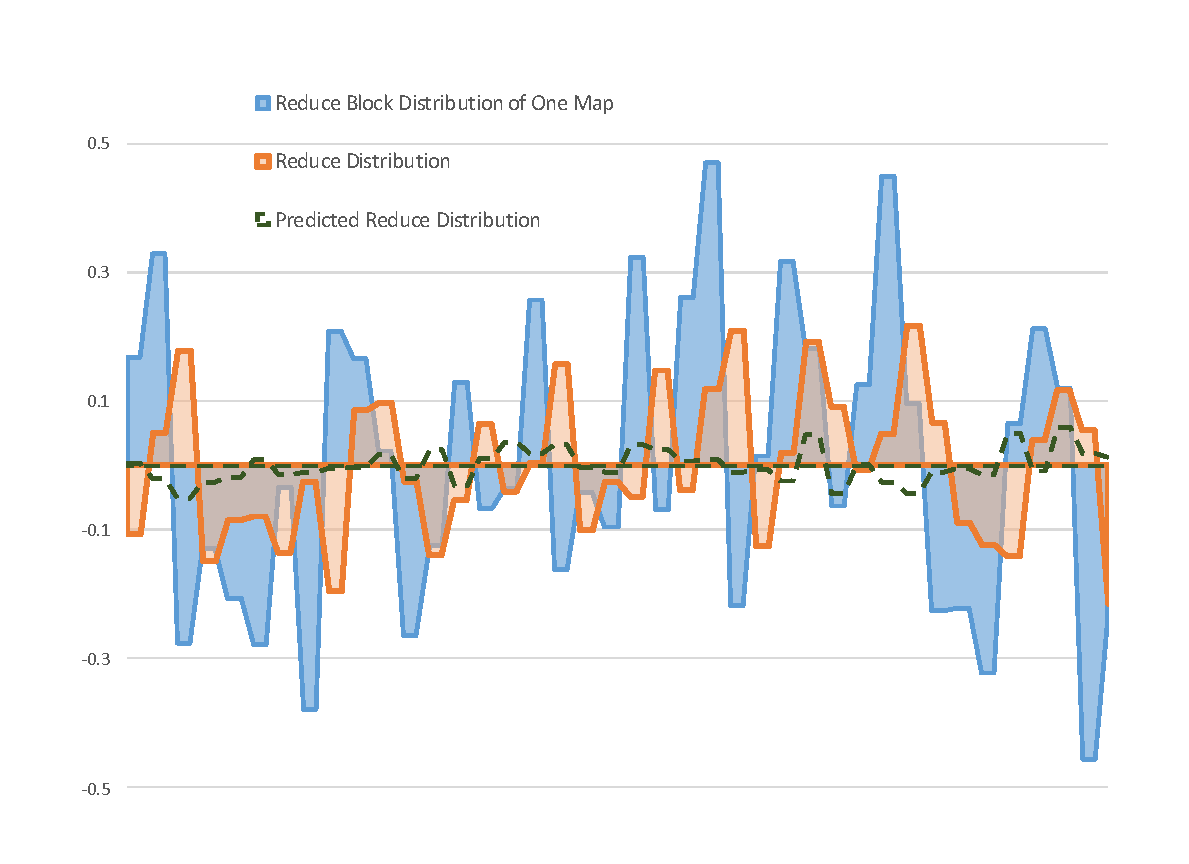
\includegraphics[width=\linewidth]{fig/range_pre_random}
		\caption{Reduce Distribution of Range Parition in Random Dataset}
		\label{fig:range_pre_random}
	\end{subfigure}
	\begin{subfigure}[b]{0.32\linewidth}
		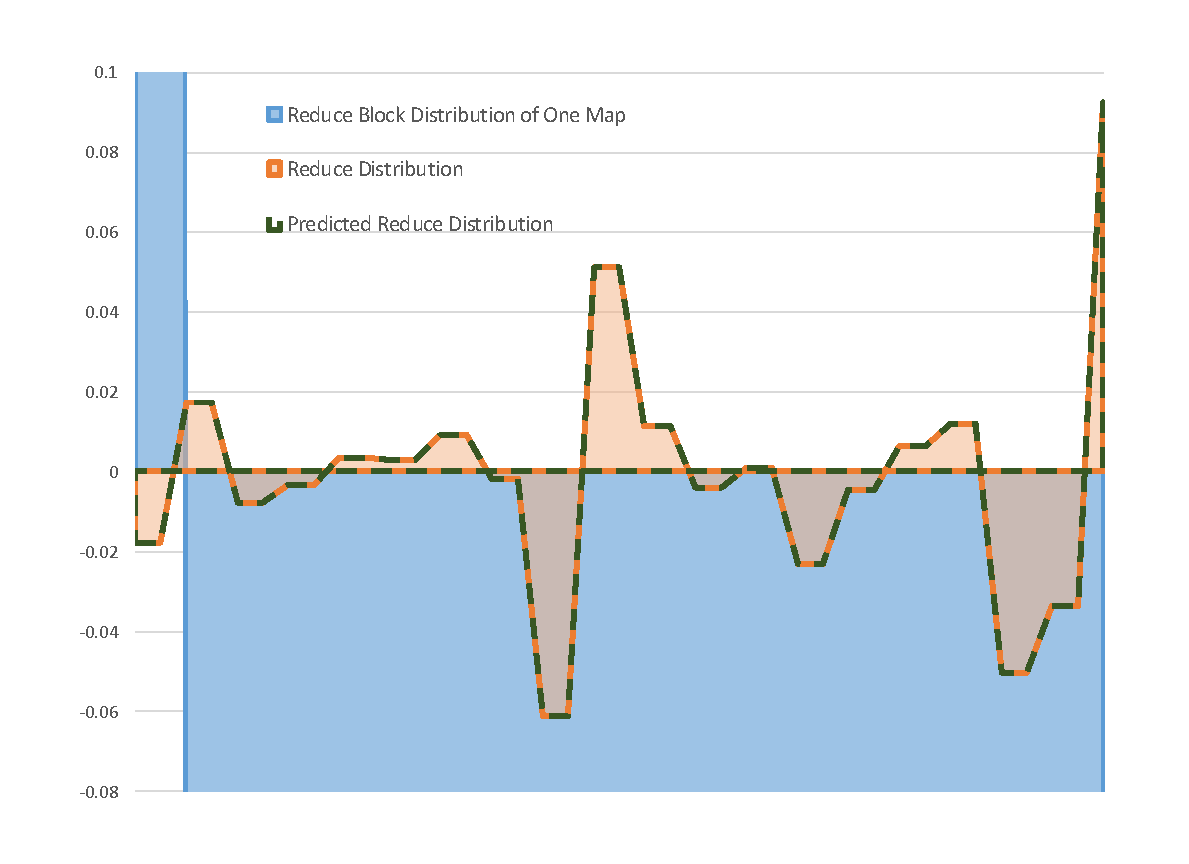
\includegraphics[width=\linewidth]{fig/range_pre}
		\caption{Reduce Distribution of Range Parition in Skew Dataset}
		\label{fig:range_pre}
	\end{subfigure}
	\caption{Reduce Distribution among Different Partition Function and Dataset}
	\label{fig:dis}
\end{figure*}
\subsection{Pre-schedule with Application Context}
Naively random map tasks to end hosts. It's bad, may skew. We have perform more balanced allocation to avoid hurting the performance of successor tasks.
Show the simulation with open cloud trace. 

In order to acheive better balanced allocation, we should combine with application context and DAG.

For one shuffle, we can use first few tasks output to predict reduce distribution such as \cite{ishuffle}. 

But results vary due to the input data distribution and partition function. Show three pics (hash parition and two range partition)

For hash partition function, in most scenrios are enough to have first completed tasks.

For range partition function and customed partition function, the relation between one output and the whole distribution can be oppsite.
To avoid complex modification, we keep the partition function as a black box and use weighted reservior sampling to prob the distribution.
Show the prediction result and accurance.

For each prediction result, a percentage array of total data composition is calculated.

Combined with DAG information, i.e. other co-existing shuffle dependencies.

present pseudo code. (not completed yet).

\section{Design}\label{design}
\section{Evaluation}

\section{Conclusion}



\bibliographystyle{abbrv}
\bibliography{biblio}

\end{document}


